
\section{在室者情報を用いた応用システムについて}\label{3.4}
部屋利用者の在室者情報を用いれば,部屋の管理者や部屋利用者にとって便利な応用システムが考えられる.
1つ目の応用システムとして,勤怠管理システムが考えられる.
勤怠管理システムの代表例としてタイムカードでの打刻や,ICカードやQRコード,スマートフォンによる記録が挙げられる.
これらのシステムでは利用者が能動的に記録する必要がある.
本研究でのビーコンを用いた手法では能動的な記録を必要とせず,自動で記録されるため,利用者の負担や記録忘れが減ると考えられる.

2つ目の応用システムとして,コミュニケーション機会の損失を減らすシステムが考えられる.
% 研究室では在室中に特定の人物がいつ来るかを
研究室では部屋利用者同士の活発なコミュニケーションが求められる.
しかし研究室内で目的とする人物と直接会うのを希望していたとしても,その人物が来るかどうかはその人にとって不明である.
会うのを希望する人に対してSNSなどのコミュニケーションツールを使っていつ頃くるかと言った連絡はできるが,仲が良い人でないとメッセージのやり取りに心理的なハードルが存在する.
そこでこれを改善する既存研究として図\ref{petgaiyou}に示す「今日の滞在」というシステムがある.
% そこで部屋利用者が共有できる情報である在室者情報を用いてコミュニケーションを促進するようなシステムがある.
このシステムでは普段の在室者の入退室情報を用いて,来そう,帰りそうという状態を予測し,その予測結果と実際の部屋の在室者と退室者の状態を提示するシステムである.
この情報をWebサイトと研究室内のディスプレイに表示し,来そう,帰りそうという表示をもとにコミュニケーション機会の損失を軽減するのが目的である.
% コミュニケーション促進システムについては4章で実装した「きょうの滞在」で詳しく述べる.

3つ目の応用システムとして,来訪促進システムが考えられる.
在室者情報を用いたゲーミフィケーションに基づくシステムが考えられる.
具体例として在室履歴を用いたペット育成ゲームが考えられる.
在室履歴を用いたペット育成ゲームの概要を図\ref{petgaiyou}に示す.
部屋利用者の在室履歴からペットに餌を与えられるようなシステムである.
部屋利用者はペットに餌を与えるためには部屋に在室する必要がある.
そのためペットに愛着があるなら部屋利用者は来訪する必要がありこれによって来訪促進が期待できる.
% また在室履歴を用いたペット育成ゲームのアプリのイメージ図を図\ref{petimage}に示す.
% 誰でも見やすいようなレイアウトやスマホでの利用を想定したボタン配置を意識した.
\begin{figure}[H]
  \begin{center}
    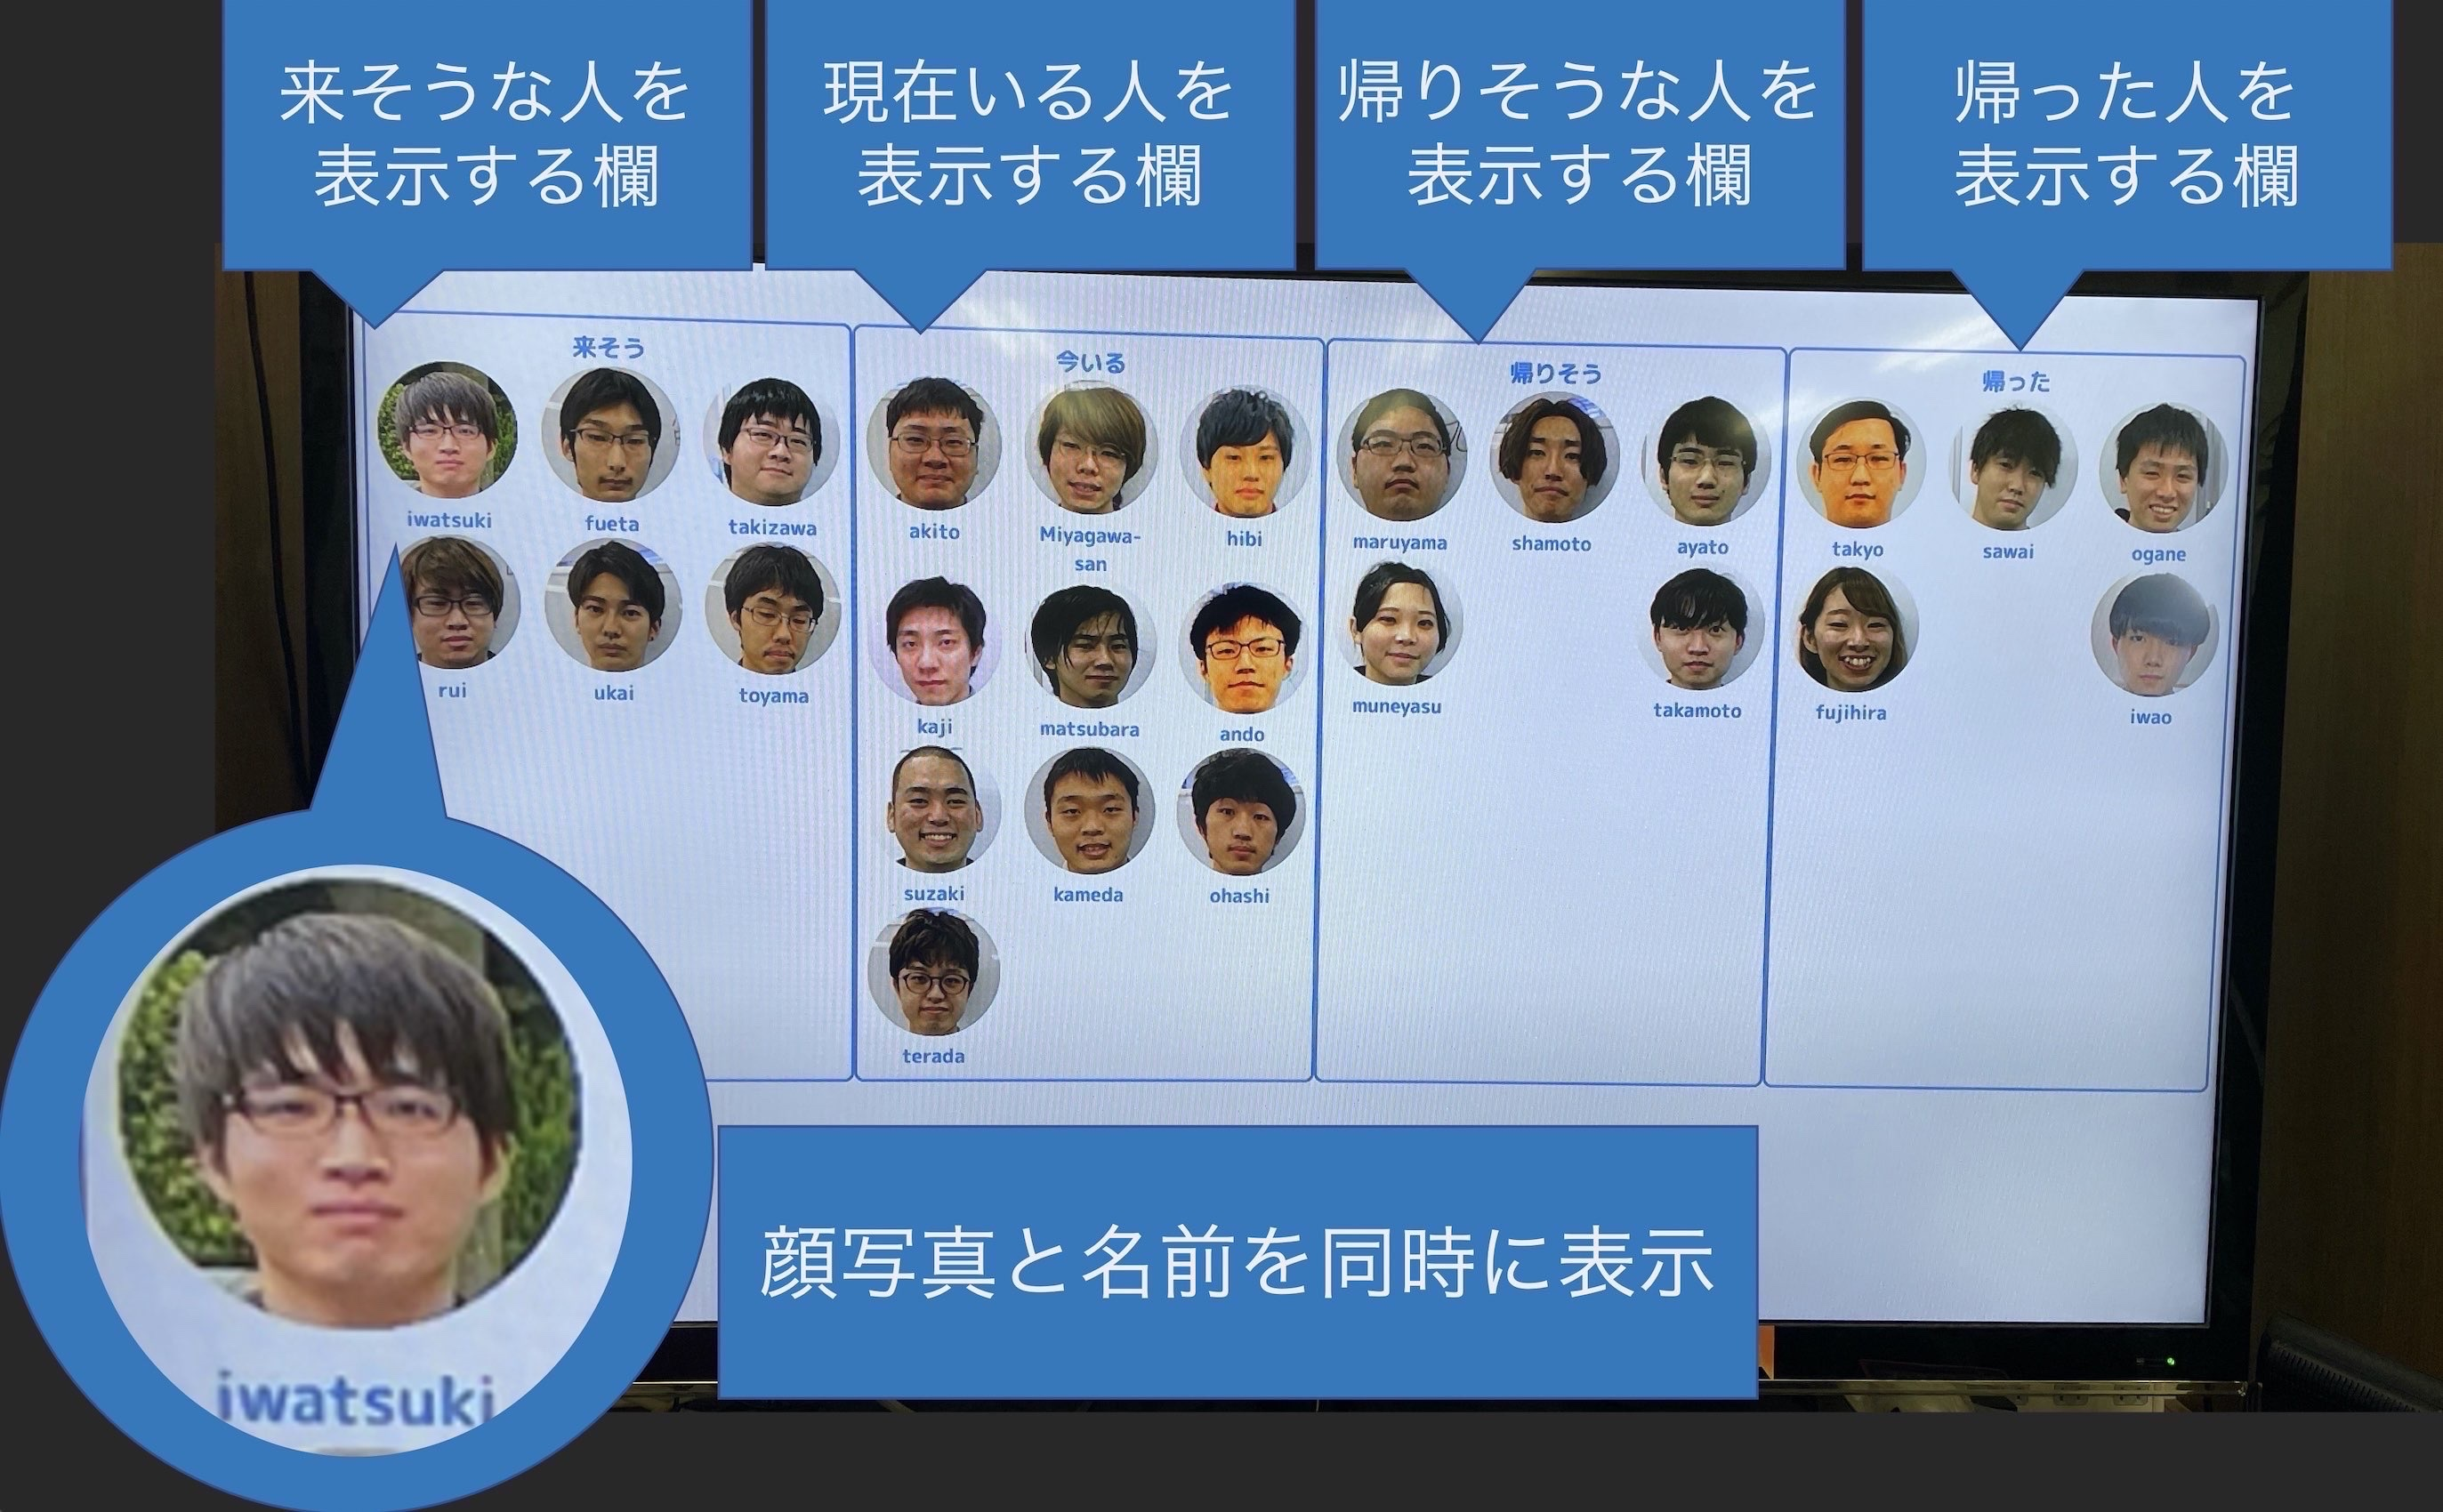
\includegraphics[width=160mm]{image/todayStay.jpg}
    \caption{コミュニケーション機会の損失を減らすシステム}
    \label{todayStay}
  \end{center}
\end{figure}

\begin{figure}[H]
  \begin{center}
    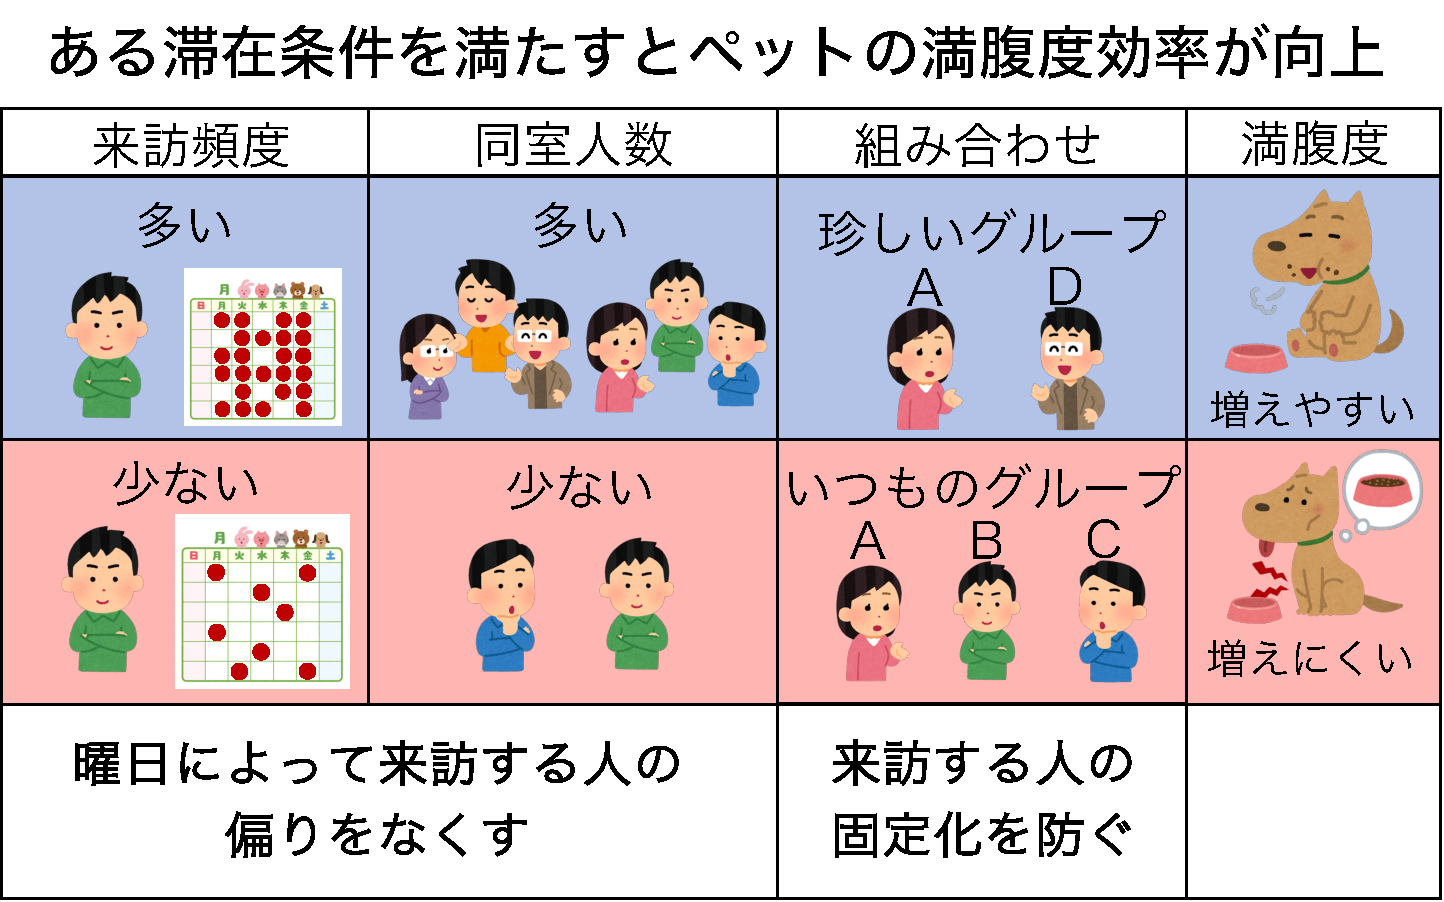
\includegraphics[width=160mm]{image/petgaiyou.pdf}
    \caption{ペット育成ゲームのアプリのイメージ}
    \label{petgaiyou}
  \end{center}
\end{figure}

\thispagestyle{myheadings}